Το Σχήμα~\ref{fig:examples} δείχνει πραγματικές προβλέψεις από την πλήρη
εκτέλεση. Για κάθε ταξινομητή επιλέγονται, με τη σειρά των δεικτών του test
set, οι πρώτες δύο σωστές και οι πρώτες δύο λανθασμένες προβλέψεις.
Η επιλογή είναι αναπαραγώγιμη και δεν αποτελεί τυχαίο ή αντιπροσωπευτικό
δείγμα της συνολικής απόδοσης. Τα ονόματα παραμένουν στην αγγλική μορφή
του CIFAR-100 για άμεση αντιστοίχιση με τα μεταδεδομένα.

\begin{figure*}[t]
\centering
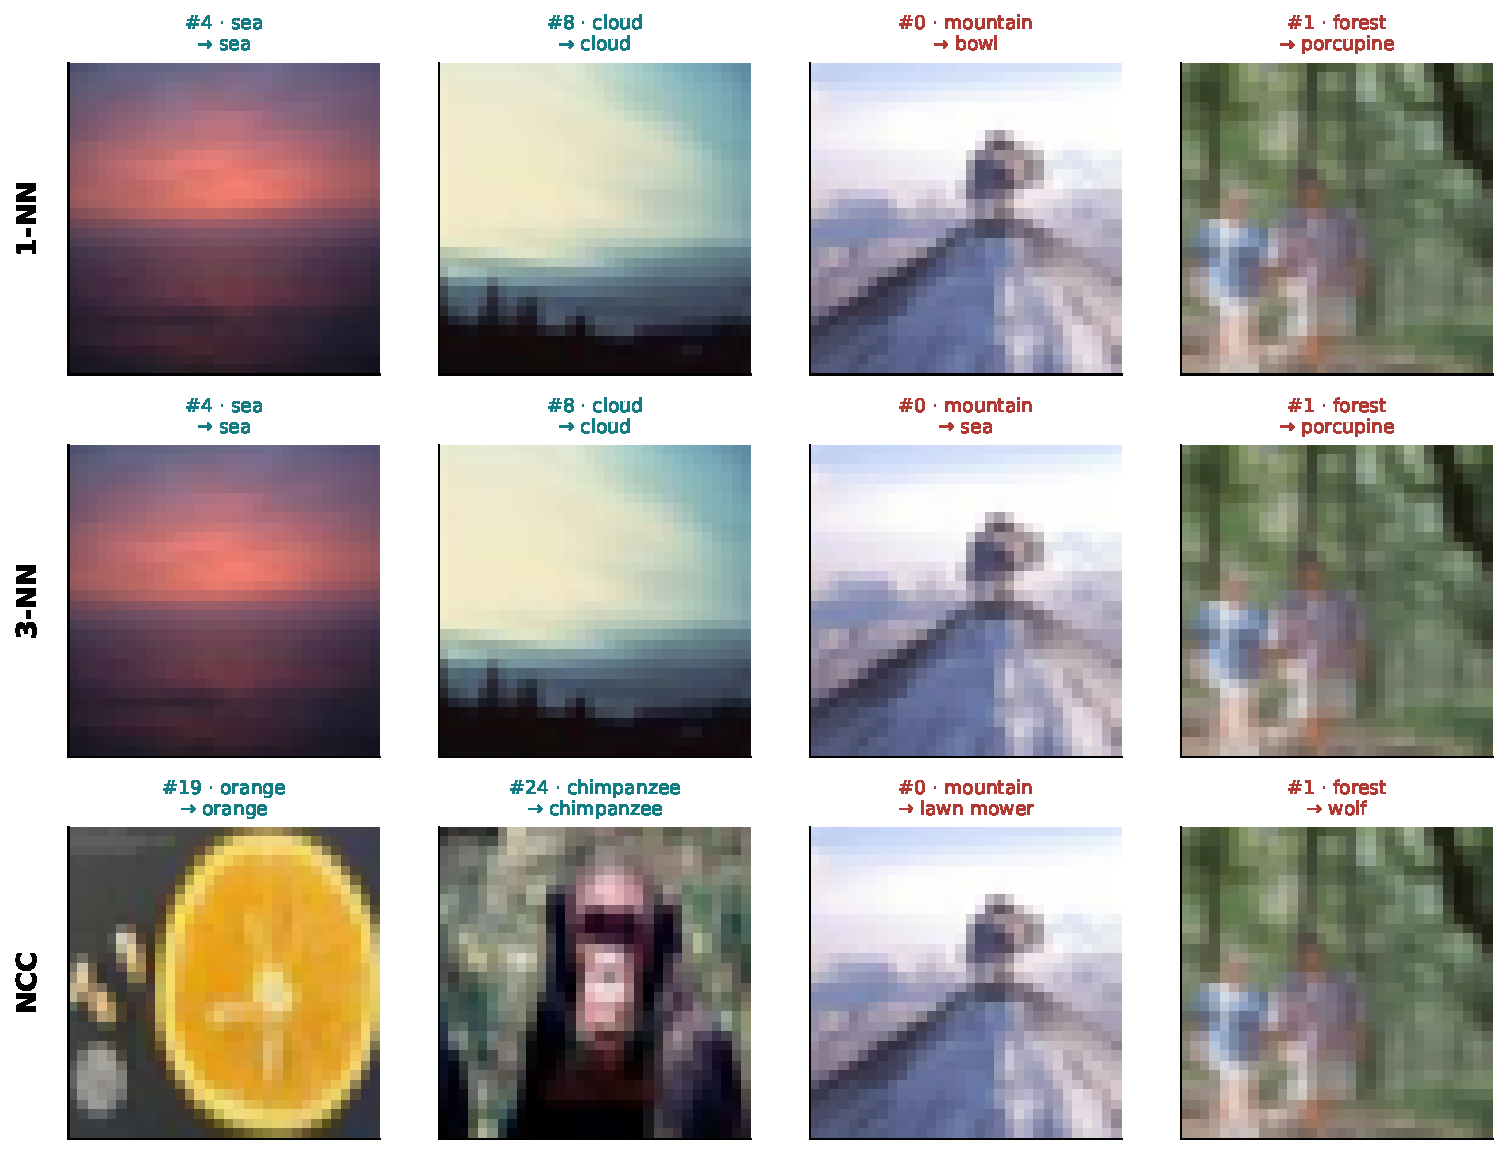
\includegraphics[width=0.95\textwidth]{figures/classification_examples.pdf}
\caption{Μία σειρά ανά ταξινομητή. Οι δύο αριστερές στήλες είναι σωστές
προβλέψεις (πράσινοι τίτλοι), οι δύο δεξιές λανθασμένες (κόκκινοι τίτλοι).
Πάνω από κάθε εικόνα αναγράφονται ο δείκτης στο test set και η πραγματική
κλάση· μετά το βέλος ακολουθεί η πρόβλεψη.}
\label{fig:examples}
\end{figure*}
